\documentclass[pdftex,12pt,a4paper]{article} 
% margin size
\usepackage[margin=1in]{geometry}

% Math and algorithms
\usepackage{amsmath,amssymb,amsthm,esint}  % For both in-line and equation mode
\usepackage{bbm}
\usepackage{bm}
\usepackage{algorithm}
\usepackage{algorithmic} % Algorithm styles, need to be nested for the example shown
\usepackage{aliascnt}
\numberwithin{equation}{section} % Numbering of our equations per section
\newtheorem{theorem}{Theorem}
\newtheorem{definition}{Definition}
\newtheorem{proposition}{Proposition}
\newtheorem{corollary}{Corollary}
\newtheorem{remark}{Remark}

\usepackage{setspace} %Spacing on the front page for crest and titles
\usepackage[]{fncychap} % Styles can be Sonny, Lenny, Glenn, Conny, Rejne, Bjarne and Bjornstrup
\usepackage[hyphens]{url} % Deals with hyphens in urls to make them clickable
\usepackage{xcolor} % Great if you want coloured text

% Figures
\usepackage{graphicx} % Inserting images
\graphicspath{ {../figures/} } 

% Tables
\usepackage{tabularx}
\usepackage{multirow} 
\renewcommand{\arraystretch}{1.5}

% Appendix
\usepackage{appendix} 

\usepackage{natbib}
\usepackage{comment}

% Tikz figures
\usepackage{tikz}
\newcommand{\ImageWidth}{14cm} 
\usetikzlibrary{decorations.pathreplacing,positioning, arrows.meta} 

 % Fancy headers and footnotes
 \usepackage{fancyhdr}
\usepackage[symbol]{footmisc}
\renewcommand{\thefootnote}{\fnsymbol{footnote}} 

% Hyperlinks and auto-references
\usepackage[hidelinks]{hyperref}  
\def\sectionautorefname{Section}
\def\appendixname{Appendix}
\newcommand{\propositionautorefname}{Proposition}
\newcommand{\definitionautorefname}{Definition}
\newcommand{\corollaryautorefname}{Corollary}  

%%%%%%%%%%%%%%%%%%%%%%%%%% DOCUMENT STARTS %%%%%%%%%%%%%%%%%%%%%%%%%%%%% 

\begin{document} 
% Front page 
%\pagestyle{empty} 

% Warwick Crest
\begin{center}
	
\includegraphics[scale = 0.5]{preamble/warwick-crest.pdf} 
\end{center}
\vspace{5mm}

% Dissertation Title
\begin{center}
	\textbf{\begin{huge}
		Why Do Men Keep Swiping Right?\\ 
		\vspace{0.2mm}
		Two-Sided Search in Swipe-Based Dating Platforms 
	\end{huge}} 
	\vspace{8mm}
\end{center}

% Author
\begin{center}
	\textbf{\large Patricio Hernandez Senosiain\footnote[1]{I am immensely grateful to Dr. Jonathan Cave for his supervision throughout the course of this project, during which he provided invaluable advice and support.}}
	
\end{center}

% Supervisor, Department and Date
\begin{center}
	%{\large Supervisor: Dr. Jonathan Cave}\\
	%\vspace{5mm}
	\textbf{\large Department of Economics}\\ 
	{\large April 2022\\}
	\vspace{10mm}
\end{center} 

% Abstract
\begin{center}
	%\section*{Abstract}
%\addcontentsline{toc}{section}{Abstract} 
\begin{abstract}
    \noindent In today's love market, swipe-based dating platforms (SBDPs) such as Tinder or Bumble have a well-established presence, but novel platform features can add significant complexities to the user's search problem in ways that have been largely under-studied in existing literature.
    This paper formulates a model of two-sided matching within SBDPs, where agents with heterogeneous preferences search for multiple romantic partners whilst facing intertemporal action constraints.
    Using numerical methods, I approximate equilibria at the steady-state and perform comparative statics on exogenous model parameters that help explain stylised empirical facts.
    Finally, agent-based simulations are used to asses the structure of steady-state equilibria as well as its attainability under myopic best-response dynamics.  
\end{abstract}
%\vspace{1cm}
%\noindent \textit{Keywords: Flux Capacitor, 1.21 Gigawatts, Calvin Klein}
\end{center} 
\vspace{5mm}




  
\begin{titlepage}
    \title{Why Do Men Keep Swiping Right? Two-Sided Search in Swipe-Based Dating Platforms\thanks{I am immensely grateful to Dr. Jonathan Cave for his supervision throughout the course of this project, during which he provided invaluable advice and support.}}
    \author{Patricio Hernandez Senosiain\thanks{Contact: \href{mailto:hdzsen.patricio@gmail.com}{hdzsen.patricio@gmail.com}. All code produced for this project is available under GitHub repository \href{https://github.com/patohdzs/project-swipe}{\texttt{patohdzs/project-swipe}}}}.
    \date{\today}
    \maketitle
    %\section*{Abstract}
%\addcontentsline{toc}{section}{Abstract} 
\begin{abstract}
    \noindent In today's love market, swipe-based dating platforms (SBDPs) such as Tinder or Bumble have a well-established presence, but novel platform features can add significant complexities to the user's search problem in ways that have been largely under-studied in existing literature.
    This paper formulates a model of two-sided matching within SBDPs, where agents with heterogeneous preferences search for multiple romantic partners whilst facing intertemporal action constraints.
    Using numerical methods, I approximate equilibria at the steady-state and perform comparative statics on exogenous model parameters that help explain stylised empirical facts.
    Finally, agent-based simulations are used to asses the structure of steady-state equilibria as well as its attainability under myopic best-response dynamics.  
\end{abstract}
%\vspace{1cm}
%\noindent \textit{Keywords: Flux Capacitor, 1.21 Gigawatts, Calvin Klein} 
    \setcounter{page}{0}
    \thispagestyle{empty}
\end{titlepage}  

% Contents page
%\renewcommand{\headrulewidth}{0pt} 
\tableofcontents
\clearpage
\renewcommand{\thefootnote}{\arabic{footnote}}
\pagestyle{fancy}
\fancyhf{}
\setlength{\headheight}{14.49998pt}
\addtolength{\topmargin}{-2.49998pt} 
\lhead{Why Do Men Keep Swiping Right?}
\def\layersep{2.5cm}
\pagenumbering{arabic}
\lfoot{\centering \thepage}
\onehalfspacing 


\section{Introduction}
\label{sec:section1}
It is widely acknowledged that the search for love is a complex social phenomenon, but in today's world, swipe-based dating platforms (SBDPs) seem to only make it trickier.
These platforms, exemplified by Tinder, Bumble, and Hinge, provide a gamified way of browsing through potential romantic partners by swiping through a stack of suggested candidates to indicate likes or dislikes for these, one profile at a time.  
In the search and matching literature, settings like these fall under the category of decentralised two-sided matching markets \citep{kanoria2021facilitating} and, despite broad differences with traditional dating sites that perform centralised static matching, SBDPs have come to dominate the modern love market, with Tinder alone boasting 75 million monthly active users and 9.6 million paid subscribers as of 2021 \citep{web:tinder_stats}.

From a theoretical standpoint, search within SBDPs induces several complexities stemming from platform-specific features, such as swiping caps, asynchronicity, and directed search algorithms.
These impose non-trivial constraints on the way utility-maximising agents strategise their search, but they have been sparsely studied in the economics literature due to the relative novelty of these platforms.
Overall, the prevalent role of SBDPs in shaping modern romantic interactions and their largely understudied nature motivates many different questions.
Nevertheless, exploring these requires a fundamental understanding of how users make decisions in these platforms: to put it simply, \textit{when should a utility-maximising user swipe right?}

This dissertation will explore the above within an SBDP setting, where agents with heterogeneous preferences on both sides of the market search simultaneously for multiple romantic partners.
Crucially, I focus on explaining (what I refer to as) the `Fast-Swiping Males' puzzle: that is, the empirical observation that men in SBDPs respond with significantly higher swipe rates and face considerably worse matching outcomes than women. This phenomenon has been both a subject of empirical research \citep{tyson2016first} and a contentious discussion point within mainstream media \citep{web:vice_tindermen, web:wp_miserabletinder}, and yet a significant gap persists within the literature for an exploration of this through a theoretical lens \footnote{Among the surveyed literature, perhaps the only partial examination of this phenomenon is provided by \cite{kanoria2021facilitating}}. 
Such analysis would add significant value since the potential causes of this phenomenon (user patience, differential preferences, and strategic dominance) are all systematically endogenous with one another, thus demanding a rigorous model that can isolate these individual effects and trace their propagation across the SBDP market.
Fundamentally, I show how gender imbalances within the platform (which arise due to several exogenous factors) can explain the above disparities and, expanding on this, I model a possible intervention where the swiping cap ratio between sexes can be set in a socially-efficient manner.

This work presents two main contributions to existing literature on the topic. 
Firstly, it constitutes one of a handful of attempts to model the market configurations arising within SBDPs, which is unsurprising due to the novelty of these platforms, but important given their current social relevance. 
Furthermore, it distinguishes itself from other similar works by directly considering the `Fast-Swiping Males' puzzle as well as the impact of swiping caps both as a constraint in the agent's search problem and a potential market correction mechanism.
Finally, this work provides an interesting case study for the use of computational methods within game theory, a field that has traditionally emphasised pure mathematical analysis.
By pairing a rigorously-formulated model with numerical computations and agent-based simulations, this dissertation exemplifies how the two approaches, rather than being mutually exclusive, can be jointly applied to complicated questions, as computational methods provide quick explorations that can serve as an intuitive stepping stone towards formalising mathematical arguments.

The remainder of the paper is structured as follows. In \autoref{sec:section2}, I outline the theoretical framework for the model developed in this paper, and derive necessary conditions for both the platform steady state and agent best-responses. In \autoref{sec:section3}, I present a refined definition for the steady-state equilibrium of the model and perform computational comparative statics on several parameters, with the aim of replicating stylised empirical facts and explaining the `Fast-Swiping Males' phenomenon. In \autoref{sec:section4}, I utilise agent-based simulations to analyse the convergence and dynamics of my model, and present a discussion on socially-efficient budget interventions. Finally, \autoref{sec:section5} presents concluding remarks and outlines potential avenues for future research.

\subsection{Related Work}
The present work draws inspiration from two key branches of economics literature: that of search and matching theory, which studies the decision-making process of agents who seek, for example, a job, a business partner, or a spouse, and that of mean-field game theory, which models complex dynamic games involving a large number of players. 
I discuss each of these in turn, and then contrast this work with the handful of papers that have focused on specifically analysing SBDP markets.

Despite the abundance of papers within the search and matching literature, which has been amply surveyed by \cite{chade2017sorting}, I draw focus on works encapsulating the three defining features of SBDP markets: decentralised matching, two-sidedness, and non-transferable utility. 
A seminal paper at this intersection is that of \cite{burdett1997marriage}, which studies the marriage market for ex-ante heterogeneous agents under uniform random search, extending the work of \cite{becker1973theory} by showing that positive assortative matching can arise even in the absence of log-supermodularity.
Several extensions follow from this, considering idiosyncratic preferences \citep{burdett1998two}, noisy attractiveness observations \citep{chade2006matching}, and even convergence onto the set of stable matchings \citep{adachi2003search}. 
The framework outlined in this dissertation is perhaps most similar to that of \cite{burdett1998two}, with three major differences between the two. 
Firstly, the model developed in this paper extends the above by allowing for multiple partners within an agent's lifetime, a feature which was probably not significant within the labour market context considered by \cite{burdett1998two}, but which is nevertheless quintessential of SBDPs given their role in fomenting casual relationships.
Furthermore, I extend the work of \citeauthor{burdett1998two} by allowing for sex-specific mass differences in the platform, as well as exogenous agent arrival flows; a point that was of noted interest for the authors themselves, and which is fundamental when considering the effects of gender imbalances within the platform. 
Finally, the model in this dissertation adopts a discrete time framework, departing from \cite{burdett1998two} and most of the recent matching literature. 
Although continuous-time models provide sharper analysis and more flexible empirical specifications \citep{burdett1999long}, this modelling choice lends itself naturally to the use of agent-based simulations, which are used to explore equilibria convergence and dynamics in a richer manner.

On the other hand, mean-field game theory focuses on dynamic games with a large number of agents, for which curses of dimensionality arise due to intractable state spaces. 
Mean-field models tackle this issue by conditioning gameplay on the \textit{invariant state distribution}, rather than tracking the individual state of each opponent \citep{light2022mean}.
This simplifying assumption is cemented by a \textit{consistency check}, such that equilibria arise when rational play conditional on an aggregate state maintains this same state as a fixed point. 
This approach, perhaps first considered by \cite{jovanovic1988anonymous} and \cite{hopenhayn1992entry}, has been successfully applied to settings such as network routing \citep{calderone2017markov}, dynamic auctions with learning \citep{iyer2014mean} and, perhaps most relevantly, online matching platforms \citep{kanoria2021facilitating,immorlica2021designing}.
In this paper, I rely on mean-field assumptions to abstract away from observability considerations: within SBDPs, the market history is unknown to players, therefore concepts such as Perfect Bayesian Equilibrium would require players to maintain and update beliefs over history spaces, and even beliefs over the beliefs of other players(a complication known as nested beliefs \citep{brandenburger1993hierarchies}).
This yields two central problems: first, that agent strategies and equilibria become virtually impossible to compute, and, by extension, that the model assumes an unreasonable level of rationality on behalf of agents \citep{iyer2014mean}.
Thus, by conditioning interactions on the stationary platform state only, the model in this paper characterises equilibria that are both insightful and representative of real-life behaviour and dynamics. 

Among the few papers specifically considering SBDPs, \cite{kanoria2021facilitating} propose a dynamic two-sided model with vertically-differentiated agents, and show that platforms with unbalanced markets can improve welfare by forcing the short side to `propose' in all interactions. 
Furthermore, \cite{immorlica2021designing} focus on the problem of designing a directed search algorithm for SBDPs by endogenising type-contingent meeting rates for agents. 
Both of these papers present theoretical models with similar features, and these have largely influenced my work in several ways; for example, by exemplifying how a mean-field approach could greatly simplify the SBDP market from a game-theoretical perspective. 
Despite this, the above papers all model settings with one-to-one matchings only, thus differing fundamentally with my work in terms of the nature of endogeneity for agent departures. On one hand, this modelling choice makes their work and insights applicable to a wider variety of online matching platforms (such as AirBnb, TaskRabbit, etc.), but it also fails to capture an essential aspect specific to SBDPs that could have significant behavioural implications. Other than this, the main difference between my work and theirs is mostly one of perspective: whilst the above papers focus mostly on the optimal design of platform features (through mechanisms such as information constraints or directed search algorithms), I instead seek to explain, from first-principles, how empirically-observed phenomena arises in SBDPs.
\section{Theoretical Model}
\label{sec: figs tables algos}
\subsection{Setup} 
Consider the two-sided search market formed by the Tinder platform with both male and female agents looking for potential partners. For ease of exposition, we assume that this market is heteronormative such that male agents search exclusively for female agents only and vice-versa. Time is discrete and indexed $t=0,1,...$ over an infinite horizon. At every time period, agents from each sex are paired up and presented a suggested partner from the opposite side of the market. To their knowledge, this happens randomly in an unknown manner. Agents can then choose whether to swipe left (dislike) or right (like) on their suggestion, yielding an action space of $\mathcal{A}_m=\mathcal{A}_w=\{ \text{left},\; \text{right}\}$. If both agents swipe right on one another, they are said to have \textit{matched} and both receive a matching payoff, however, if either agent swipes left, they both receive a payoff of zero. Importantly, the suggested partner’s action is only \textit{observable} if one swipes right.

Each agent has an attractiveness type $\theta \in \Theta := [0,1]$ which is unknown to them but observable to their suggestion, and it is common knowledge that this is the case. Contingent on matching with a suggestion of attractiveness $\theta$, a user earns a matching payoff of $u(\theta)$, where $u(\cdot)$ is a strictly increasing, concave function that satisfies $u(0) = 0$. This last property stems from the fact that, in Tinder, users are allowed to unmatch with each other, thus implying that matching with the least attractive individual on the other side of the market is weakly preferred to the payoff from not matching. Given the above, Tinder makes right-swiping costly by placing a cap on the total number of right swipes for each user. We refer to the total number of right-swipes a user has left as its \textit{budget}, $b_t$, which evolves dynamically according to the law of motion:
$$
  b_{t+1}= b_{t}- a_{t}
$$
where the starting budgets for each sex, $B_{m}$ and $B_{w}$, are determined exogenously. The budget sets for men and women are thus defined by $\mathcal{B}_{i}=\{b \in \mathbb{Z} : 0\leq b \geq B_i\}$, with $i=m,w$ respectively. 

Each period, $\lambda_m$ new men and $\lambda_w$ new women enter the platform, with their attractiveness drawn i.i.d from distributions with c.d.f’s $F_m$ and $F_w$, respectively. Importantly, agents depart from the platform in one of two ways: they can leave \textit{endogenously}, if they expend their swiping budget, or \textit{exogenously} with probability $(1-\delta)$. This admits to the interpretation of a geometrically distributed lifetime parametrized by $\delta$, and implies that users use this as a discounting factor for future payments. At any given time $t$, the masses of men and women on Tinder are denoted by $N^t_{m}$ and $N^t_{w}$, respectively. Given sample spaces $\Theta \times \mathcal{B}_{m}$ and $\Theta \times \mathcal{B}_{w}$, let $\mathbb{P}_{m}$ and $\mathbb{P}_{w}$ be the probability measures over the corresponding $\sigma$-algebras. Furthermore, let $M^t,W^t:\Theta\times\mathcal{B}_{i}\rightarrow[0,1], \quad i=m,w$ be the endogenous mixed distributions over agents (male and female, respectively) in the platform. These are endogenously determined since the flow of agents into lower budget levels and eventually out of the platform depends on their swiping decisions, determined endogenously through a search process. Finally, since gender imbalances mean that not everyone might receive a suggestion, the question remains of how to decide which agents on the long side of the market get paired up. Since Tinder is fair and efficient platform, we model a frictionless matching technology and denote market tightness, ie. the probability of receiving a suggestion on either side, by:
$$
\tau^t_m=\min\{\frac{N^t_w}{N^t_m} ,1\}, \ \tau_w= \frac{N^t_m}{N^t_w}\tau^t_m
$$


Given the above, a number of simplifications to the explored setting are possible. 

- 1. An agent’s decision on any given time period depends fundamentally on the attractiveness of the suggested partner and their own budget

I restrict attention to stationary Markov strategies, defined by $\sigma_m: \Theta \times\mathcal{B}_m\rightarrow \Delta\mathcal{A}_m$ for men and $\sigma_w:\Theta \times\mathcal{B}_w\rightarrow \Delta\mathcal{A}_w$ for women, where $\Delta S$ is used to denote the probability simplex over set S. 

\begin{figure}[h]
    \centering
        \begin{tikzpicture}
            % draw horizontal line   
        \draw[thick, -Triangle] (0,0) -- (\ImageWidth,0) node[font=\scriptsize,below left=3pt and -8pt]{$t$};

        % draw vertical lines
        \foreach \x in {0,1,...,13}
        \draw (\x cm,3pt) -- (\x cm,-3pt);

        \foreach \x/\descr in {4/t-2,5/t-1,6/t,7/t+1}
        \node[font=\scriptsize, text height=1.75ex,
        text depth=.5ex] at (\x,-.3) {$\descr$}; 

        % braces
        \draw [thick ,decorate,decoration={brace,amplitude=5pt}] (4,0.7)  -- +(2,0) 
            node [black,midway,above=4pt, font=\scriptsize] {Training period};
        \draw [thick,decorate,decoration={brace,amplitude=5pt}] (6,-.9) -- +(-1,0)
            node [black,midway,font=\scriptsize, below=4pt] {Testing period};  
    \end{tikzpicture}
    \caption{Timeline of events within each time period} \label{fig:timeline}
\end{figure}    

\subsection{The Dating Market}
\begin{itemize}
    \item Entry flows
    \item Leaves (including geometric lifetime)
    \item Masses
    \item Distribution
    \item Steady State
\end{itemize}
\subsection{The Search Problem} 
\begin{itemize}
    \item Present case for women, then say case for men follows
    \item Condition on male strategy and steady state
    \item Present Ex-interim utility maximization
    \begin{itemize}
        \item Show it reduces to a constant
    \end{itemize} 
    \item Present sequence problem
    \item Derive Bellman equation
    \item Prove uniqueness of value function and solution
    \item Derive solution
\end{itemize}
\section{Equilibrium \& Comparative Statics}
\label{sec:section3} 
\subsection{Stationary Equilibrium and Computation}\label{sec:section3.1} 
Using the framework and results above, I now present a refined definition for the steady-state equilibrium of the market: 
\begin{definition}
    A Stationary Equilibrium (SE) is a triplet $(\mu^*, \omega^*, \Psi^*)$ such that:
    \begin{enumerate}
        \item $ \mu^*(\theta,b) \text{ attains } V_m(\theta,b),$ for all pairs $\theta, b \in \Theta \times \mathcal{B}_m$, given $\omega^*,\Psi^*$.
        \item $ \omega^*(\theta,b) \text{ attains } V_w(\theta,b),$ for all pairs $\theta, b \in \Theta \times \mathcal{B}_w$, given $\mu^*,\Psi^*$.
        \item $\Psi^*$ satisfies Equations \ref{eq:ss1}, \ref{eq:ss2}, and \ref{eq:ss3} given the strategy profile $(\mu^*, \omega^*)$.
    \end{enumerate} 
\end{definition}

Intuitively, the above definition establishes two requirements that must be satisfied by an equilibrium market configuration. 
Firstly, it must be the case that $\mu^*$ and $\omega^*$ are mutual best responses given the platform state $\Psi^*$ for which, as previously outlined, a necessary and sufficient condition would have them each solve the sex-specific MDP. 
These two conditions alone demand \textit{partially rational expectations}, as per \cite{burdett1997marriage}, since they require agents to play optimally for some fixed steady-state $\Psi^*$, imposing rationality on all game aspects other than the platform state dynamics. 
Furthermore, in line with other works in mean-field game theory, a consistency check is imposed by the third condition, such that the platform state to which agents are best-responding with $(\mu^*,\omega^*)$ is sustained as a fixed point under that same strategy profile.

Although formal proofs for the existence and uniqueness of SE are outside the scope of this paper, I rely on numerical procedures\footnote{The code required to reproduce all presented analysis is accessible under the GitHub repository \texttt{patohdzs/project-swipe}, with most dependencies covered by the SciPy Stack packages.} to approximate equilibria under various exogenous settings. 
This approach has been frequently employed by related works \citep[see][]{iyer2014mean, gummadi2011optimal} as it can help uncover insights provided by mean-field models. 
To compute model equilibria, I frame the recurrence relation presented in \autoref{prop:recurrence relation}, as well as Equations \ref{eq:ss1}, \ref{eq:ss2}, and \ref{eq:ss3}, as a system of $2(|\mathcal{B}_m|+|\mathcal{B}_w|+1)$ non-linear equations, and solve this using a modified version of the hybrid Powell method, as implemented by the MINPACK 1 routine \citep{more1980user}. 
In what follows, I present SE results for a number of comparative statics experiments. 
For all of these, the exogenous settings used to calibrate the model are provided in \autoref{appx: c}, and convergence of numerical procedures was assured by computing the squared loss of the above system, which was exactly equal to zero in all cases; although the runtime required for convergence varied slightly across experiments.

\subsection{Best Response Analysis}\label{sec:section3.2} 
Using the computational procedures outlined above, a number of insights can be uncovered related to how exogenous parameters affect an agent's optimal swiping behaviour. 
The first parameter I analyse is the discount factor, which represents the probability of remaining inside the platform for an additional time period, but is often interpreted as the representative agent's patience level.
To determine the effects of changes in the discount factor, I computed the best-response policy over a range of different values for $\delta$ (using an arbitrary set of exogenous parameters), with results shown in \autoref{fig:discount-cs}. 
Evidently, as the agent becomes less patient, they `lower their standards' for potential matches in the platform, shifting their swiping curve downwards. 

\begin{figure}[ht] 
    \centering
    \caption{Comparative Statics on the Discount Factor}
    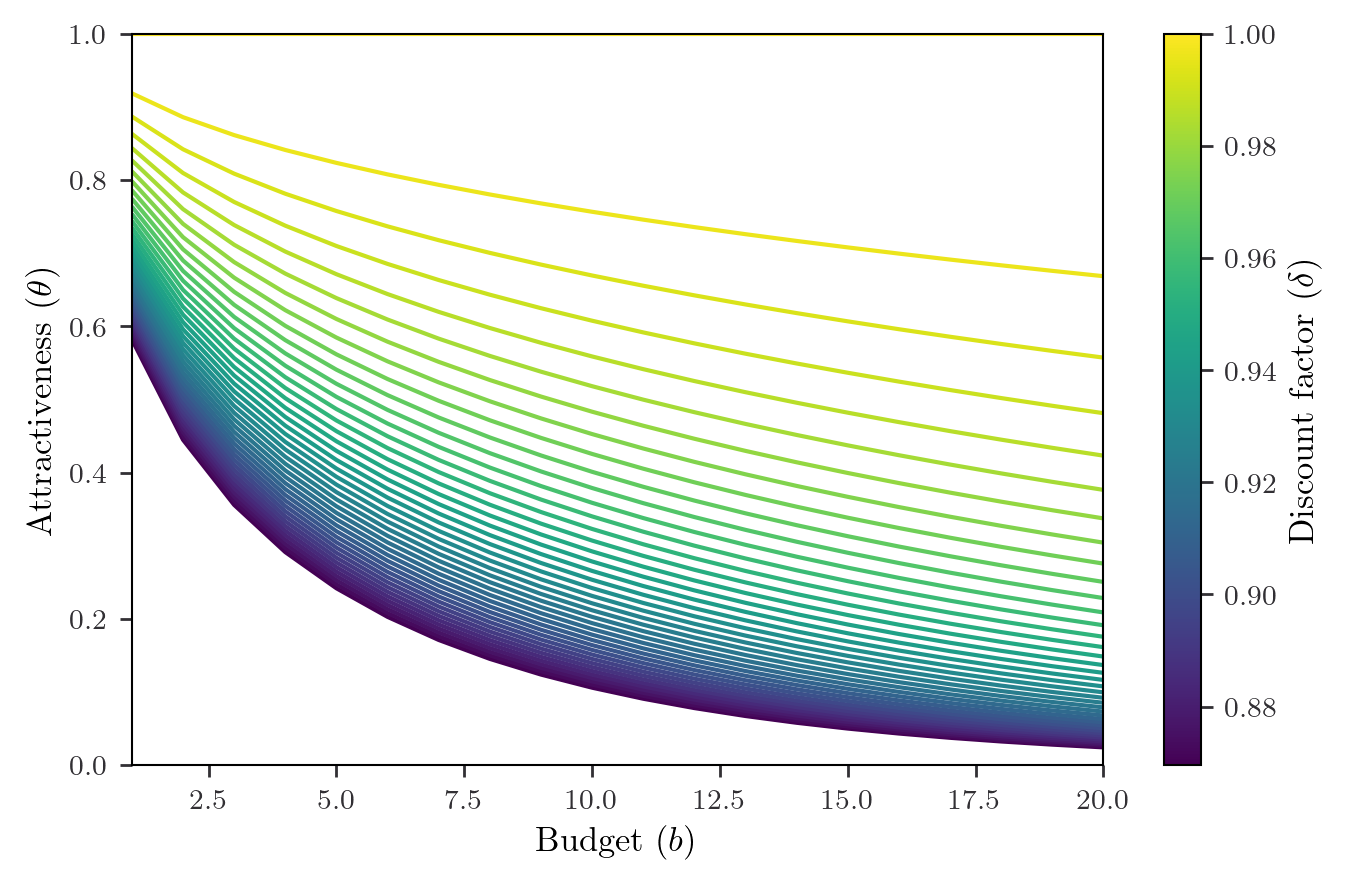
\includegraphics{discount-cs.png}
    \label{fig:discount-cs}
\end{figure} 

Another interesting parameter to examine is the absolute risk aversion of agents, which I choose to interpret as their `desperateness' for matching.
In the platform, risk-averse agents prefer a greater likelihood of matching (even if this yields relatively lower payoffs), whilst risk-loving agents prefer to save their swipes for high-yield candidates. 
To perform comparative statics on this parameter, I fix a CARA utility function for agents, with parameter $r$ corresponding to the Arrow-Pratt coefficient for absolute risk aversion. 
I then compute the optimal swiping rule for various different values of $r$, with results for this shown on \autoref{fig:risk-cs}.
From here, it is evident that as absolute risk aversion rises, agents become `more desperate' for matches, inducing them to lower their standards for right-swiping on a candidate, and thus shifting their swiping curve downwards.

\begin{figure}[ht]
    \centering
    \caption{Comparative Statics on Absolute Risk Aversion}
    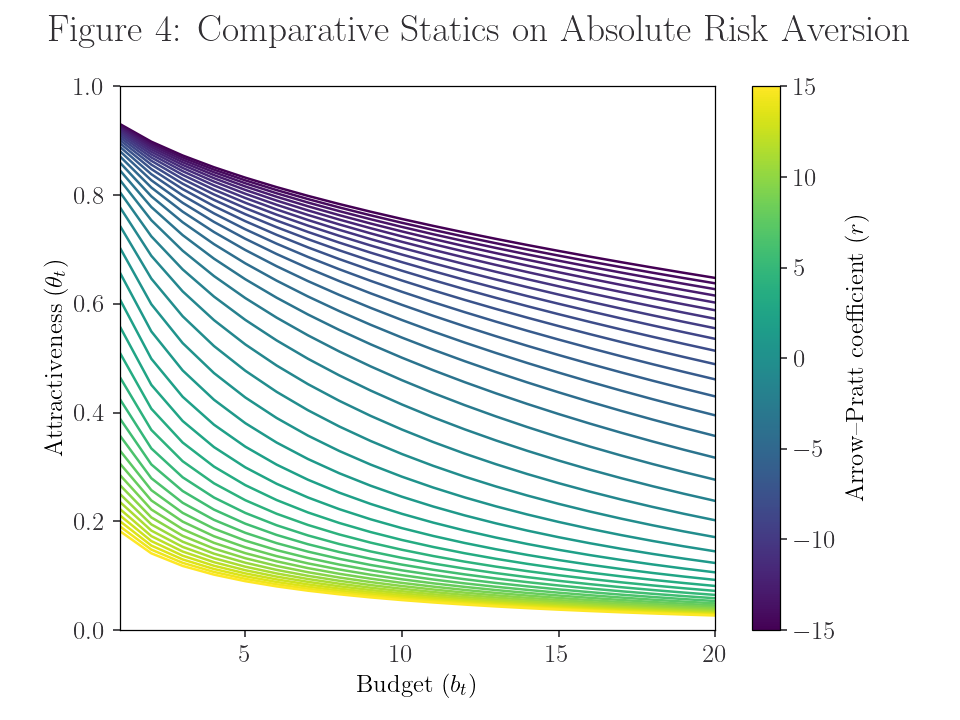
\includegraphics{risk-cs.png}
    \label{fig:risk-cs} 
\end{figure}

\subsection{Market Configuration Analysis}\label{sec:section3.3} 
Finally, I perform comparative statics at the platform level to explore how different exogenous factors affect market configurations. 
This is especially important as it considers not only the effects on best-responses for one sex, but also how these propagate across the market, ultimately affecting the other side's swiping behaviour as well. 
More specifically, I focus on the aforementioned `Fast-Swiping Men' puzzle, investigating the discrepancies in swiping rates and matching outcomes between men and women. 
There are a number of potential explanations for this behaviour, most of which concern sex-specific differential preferences which are compatible with my model. 
Indeed, it is reported that women spend around 20\% more time then men on a single Tinder session \citep{web:nytimes_patience}, potentially indicating a higher level of patience which would induce `higher standards' and a lower swiping rate, as explained above.
Departing from these, I consider below a scenario that could explain the `Fast-Swiping Men' puzzle purely as a result of tightness-induced search frictions, for which I analyse the market SE computed under a 6:1 ratio between exogenous arrival rates $\lambda_m$ and $\lambda_w$.  
This ratio was calibrated such that the steady-state mass of men in the platform is around ten times greater than that of women, in line with demographic estimates for the UK \citep{web:tinder_stats}, and results for such SE are shown in \autoref{fig:mkt-cs}. 

\begin{figure}[ht]
    \centering
    \caption{Market Configuration Under Differential Agent Inflows}
    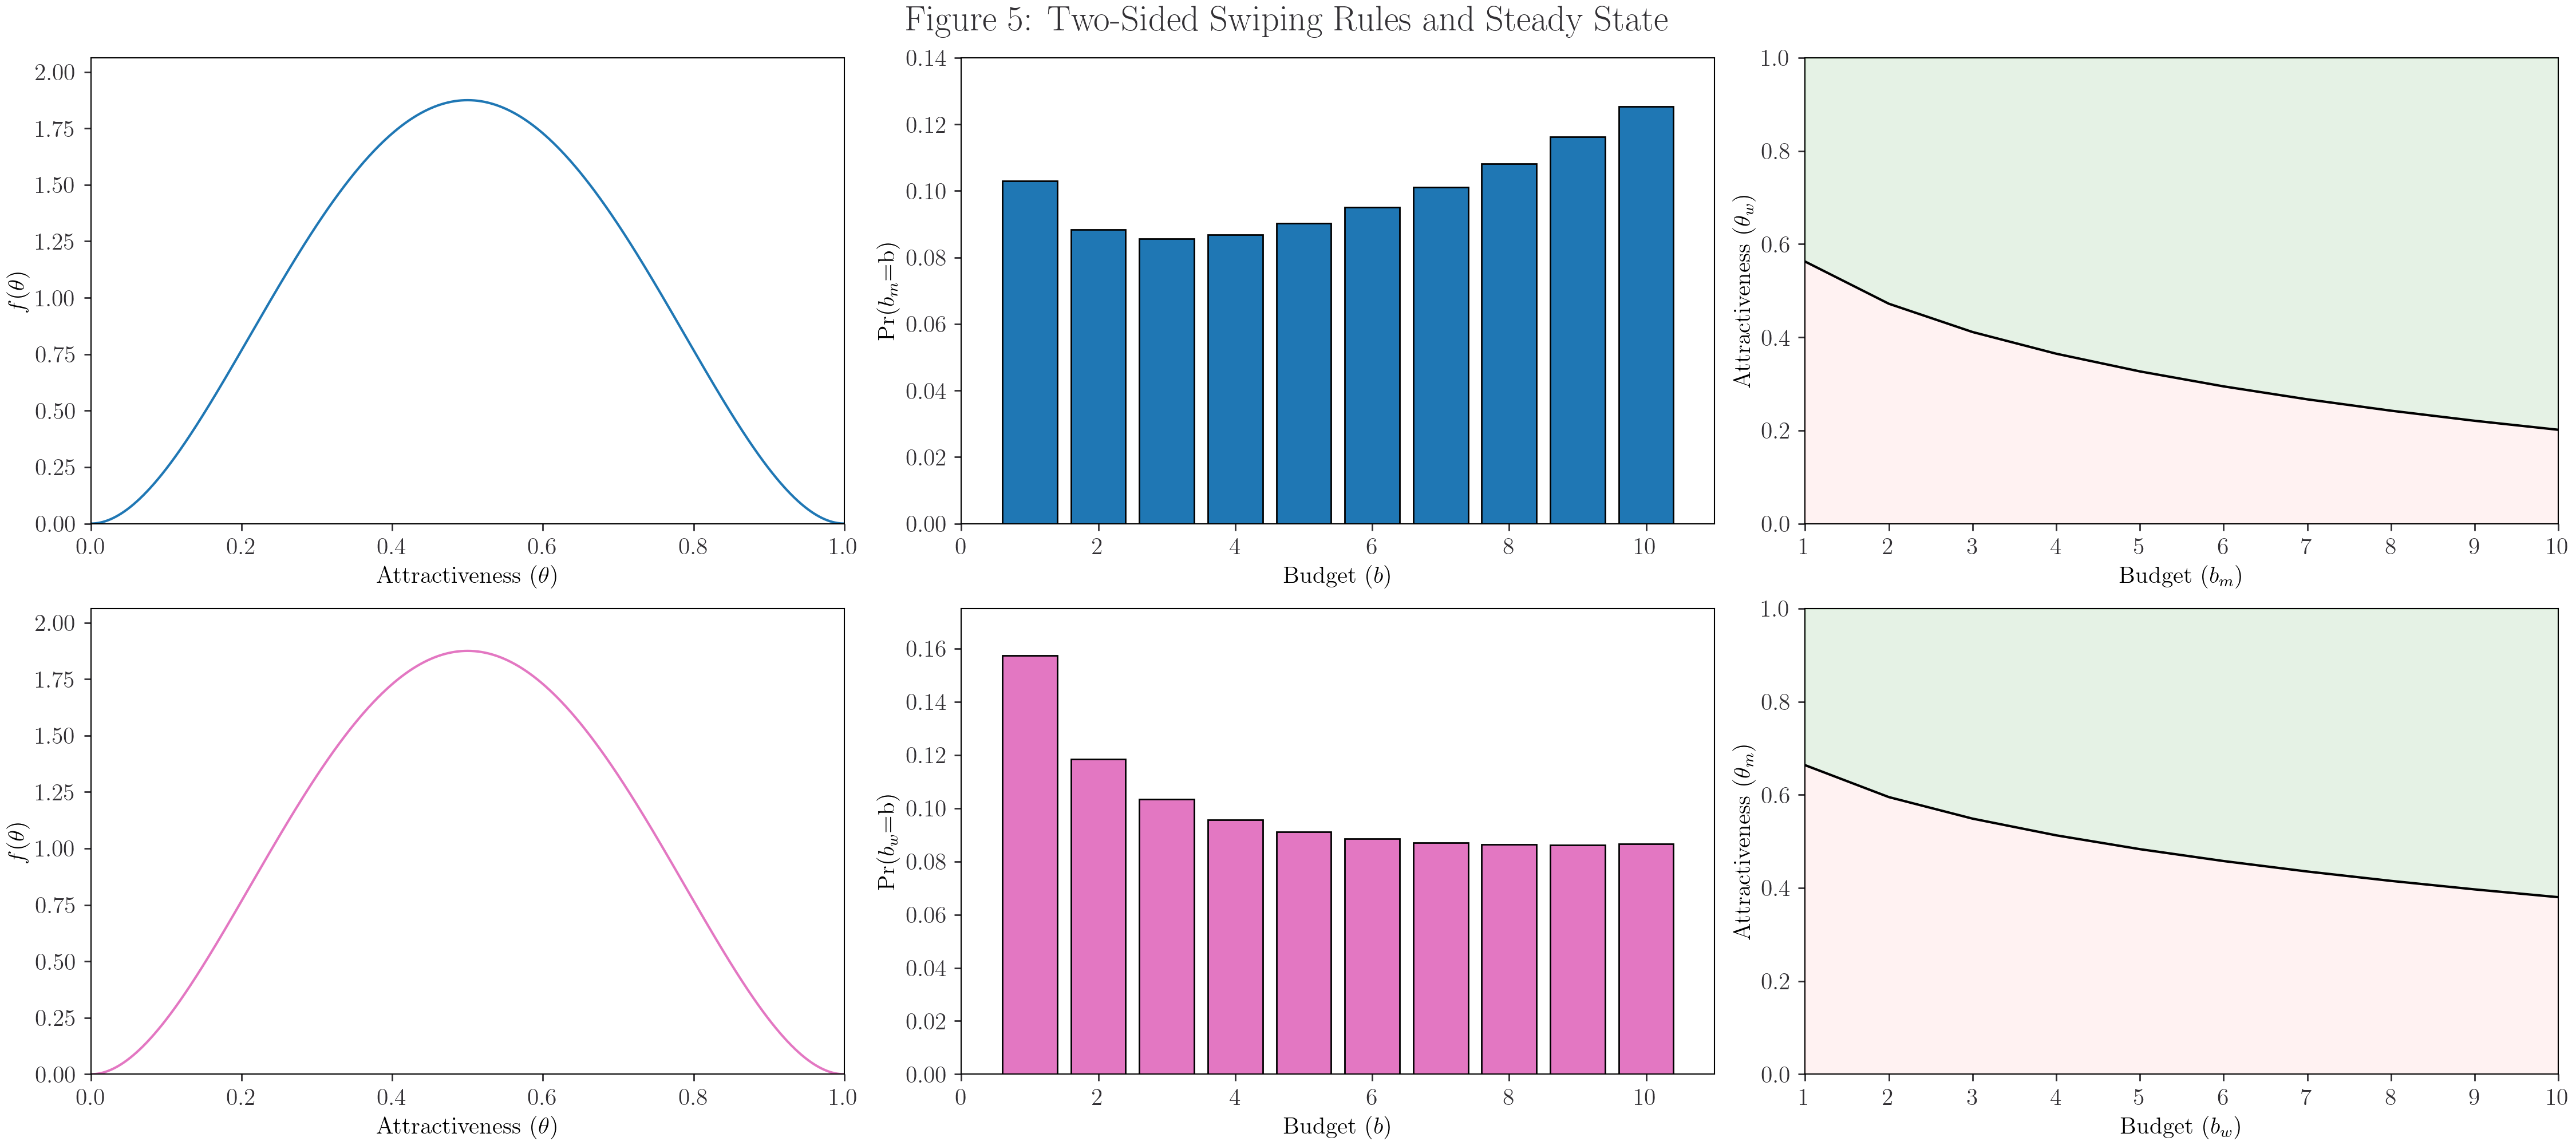
\includegraphics{mkt-cs.png}
    \label{fig:mkt-cs} 
\end{figure} 

Under the above scenario, men overcrowd the market and struggle to get paired with female candidates, evidenced by the top-center plot in \autoref{fig:mkt-cs}, which shows that male agents are highly concentrated in the top budget levels. 
Due to the effect of market tightness on the effective discount rate, male agents become more impatient than women, and this shock is absorbed by their optimal swiping policy, which sits considerably lower than the female swiping curve, effectively showing how a tight market lowers male patience and by extension, their standards, leading them to swipe right on most women. 
Ultimately, this explains the `Fast-Swiping Men' puzzle given that, under this particular SE, men swipe right with probability $\overline\mu=0.988$, compared to $\overline\omega=0.491$ for women, thus replicating the observed phenomenon. 

One potential intervention to correct this phenomenon could involve relaxing the swiping cap for the shorter side of the market.
To analyse such measure, the SE was computed under the same conditions as above but with a 4:1 swiping cap ratio between women and men; the results for this, shown in \autoref{fig:mkt-cs-bdiff}, indicate the presence of two separate effects that would help alleviate the above scenario. 
First, a larger budget set would allow women to stay in the platform for longer by shrinking the number of endogenous departures to zero (at the limit), thus leading to a larger steady-state mass of female agents that would alleviate market tightness for men. 
This is corroborated by the computed results, which show a 6:1 ratio between the male and female agent masses, down from 10:1. 
Furthermore, because optimal reservation values are decreasing in the agent's budget, women in the top budget levels would swipe right at considerably lower thresholds, thus improving matching outcomes for men. 
This is highlighted in \autoref{fig:mkt-cs-bdiff}, which shows that female swiping policy quickly descends to a level comparable to their male counterparts since it is allowed to extend over a larger budget set. 
Furthermore, under this particular SE, men swipe right with probability $\overline\mu=0.906$, compared to $\overline\omega=0.79$ for women, therefore highlighting the effectiveness of this intervention, which could be of considerable importance given both its simplicity and its potential impact on user experience, as research by \cite{kanoria2021facilitating} identifies asymmetric selectiveness as a profound source of inefficiency in dynamic matching platforms. 
\begin{figure}[ht]
    \centering
    \caption{Market Configuration Under Differential Swiping Caps}
    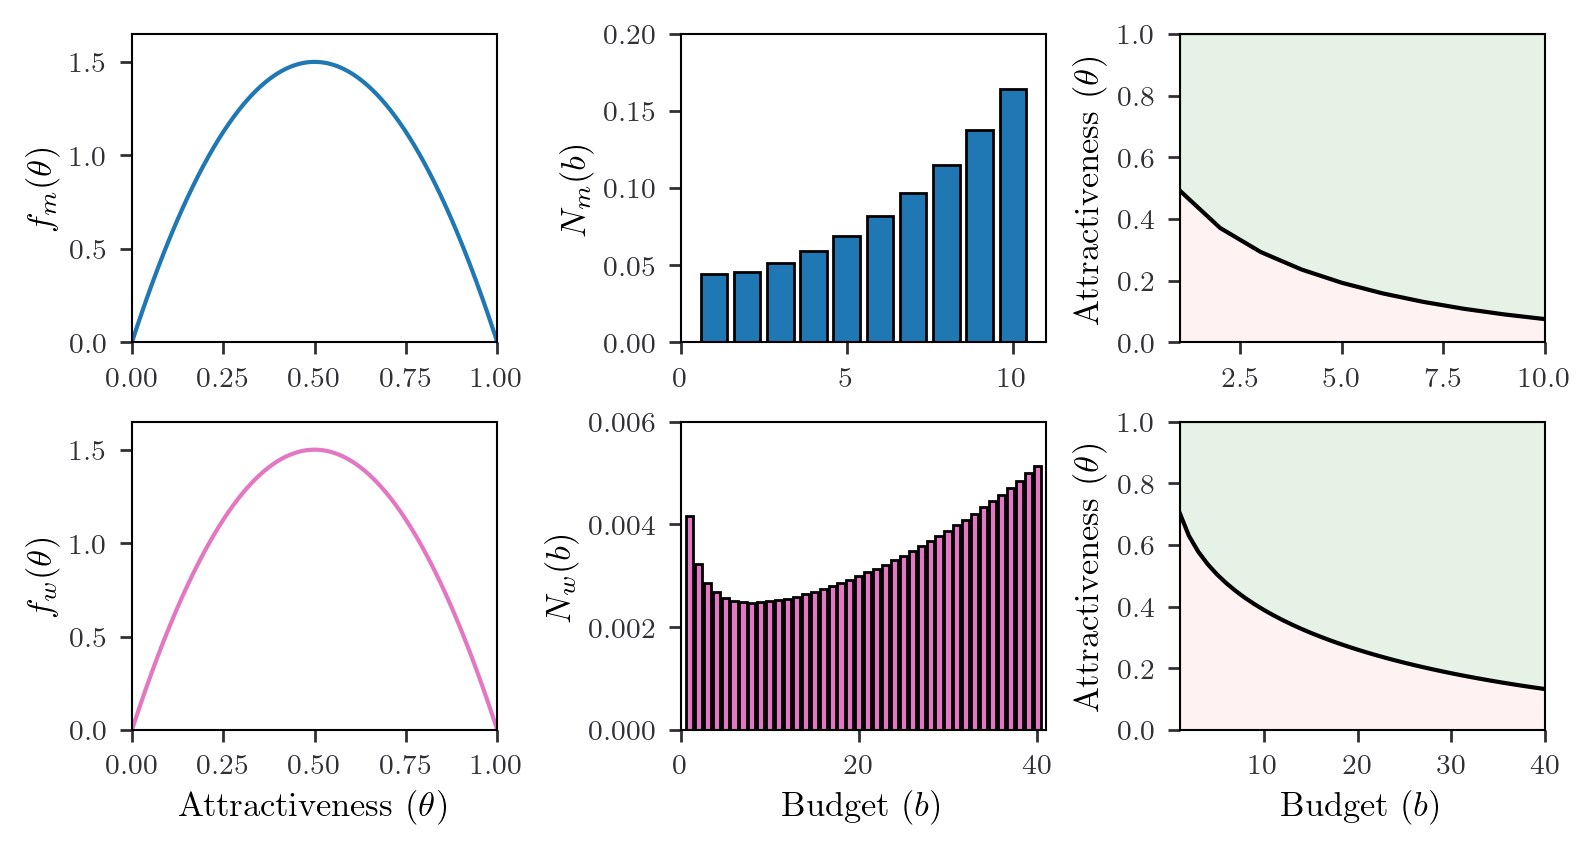
\includegraphics{mkt-cs-bdiff.png}
    \label{fig:mkt-cs-bdiff} 
\end{figure}
One potential drawback of this intervention is that general selectiveness falls in the market, since the effect prompting women to swipe more is of greater magnitude than the one prompting men to swipe less. 
This could be easily avoided by lowering the swiping cap for men, instead of raising the cap for women, to achieve the desired counterbalancing ratio, but such intervention would be inevitably bounded as the swiping cap for men approaches zero.

\section{Agent-Based Simulations}
\label{sec:section4}  
\subsection{Steady-State Convergence}
Given the lack of accessible SBDP user data, I developed on agent-based simulation environment to explore the evolution of both behavioural and market-level dynamics under the above theoretical foundation. 
Agent-based modelling (ABM) is used to study how \textit{``macro phenomena emerges from micro level behaviour among a heterogeneous set of interacting agents''} \citep{janssen2005agent}, and it has been successfully applied by recent work on matching platforms \citep{immorlica2021designing} to help identify and understand the structure of equilibria, which can be computationally expensive to approximate (and in some cases even non-existent).

\begin{figure}[ht]
    \centering
    \caption{Agent-Based Simulation Convergence}
    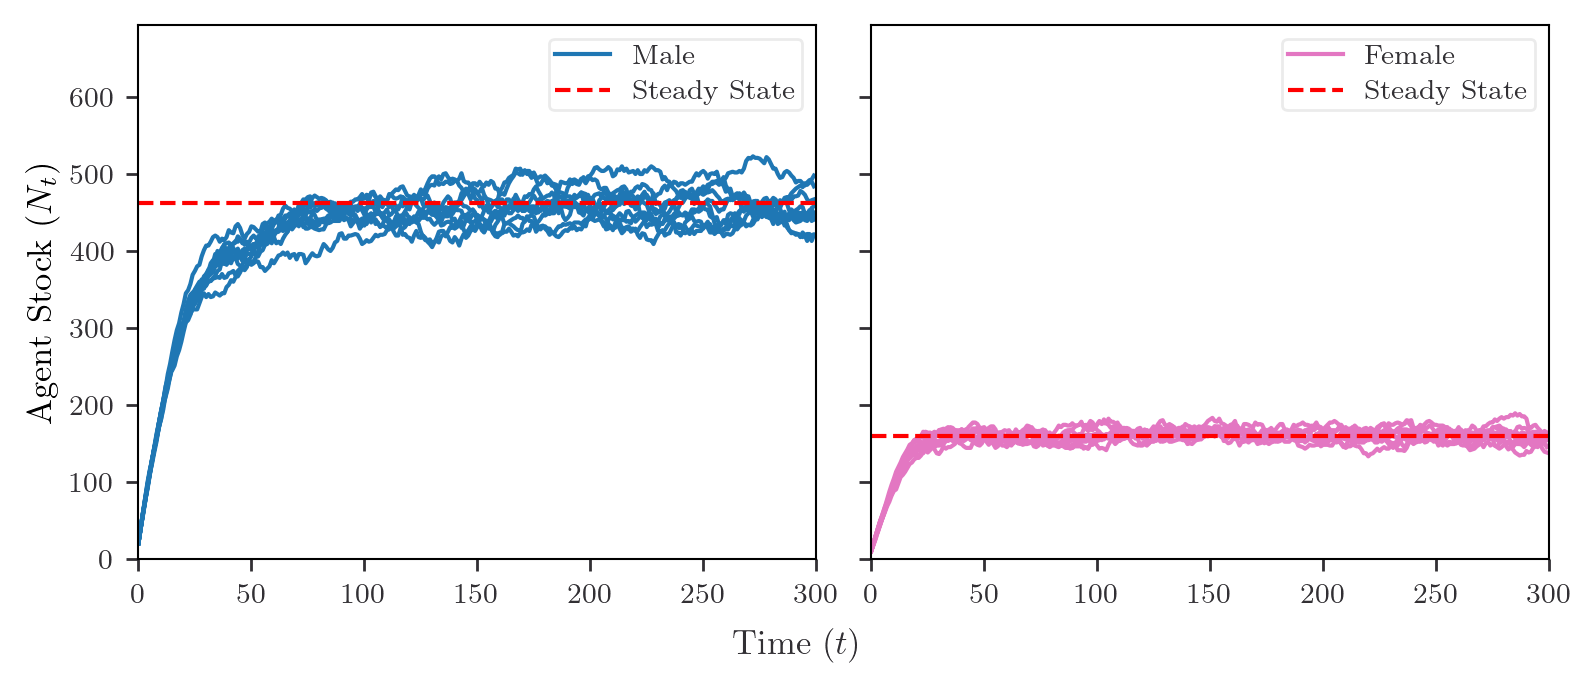
\includegraphics{abm-conv-imbalanced.png}
    \label{fig:abm-conv} 
\end{figure}

To start, I explore the convergence and stability of the SBDP market under arbitrary exogenous settings. 
In particular, \autoref{fig:abm-conv} shows the evolution of (sex-specific) agent masses for 10 independent simulation batches, over 300 time periods, and with a 2:1 ratio between male and female arrival flows. 
These simulations were conducted under partially rational expectation conditions; that is, with agents using optimal policies for some fixed steady-state even when this is not actually the current platform state.  
As evident from these results, this process converges onto the SSE computed using the procedures in \autoref{sec:section3.1}. 
Furthermore, the ABM simulations show that the long side of the market (males) takes considerably longer to converge onto its steady-state level. 
One technical point worth noting is that the above simulations involve a finite number of atomic agents as opposed to \textit{agent masses}, as per our continuum model.  
Nevertheless, I examine the limiting case of these dynamics, with \autoref{fig:abm-conv-ssize} depicting how, by the law of large numbers, stationary deviations around the steady-state level become negligible as the number of agents in the platform tends to infinity. 

\begin{figure}[ht] 
    \centering
    \caption{Agent-Based Simulation Convergence with Varying Sample Sizes}
    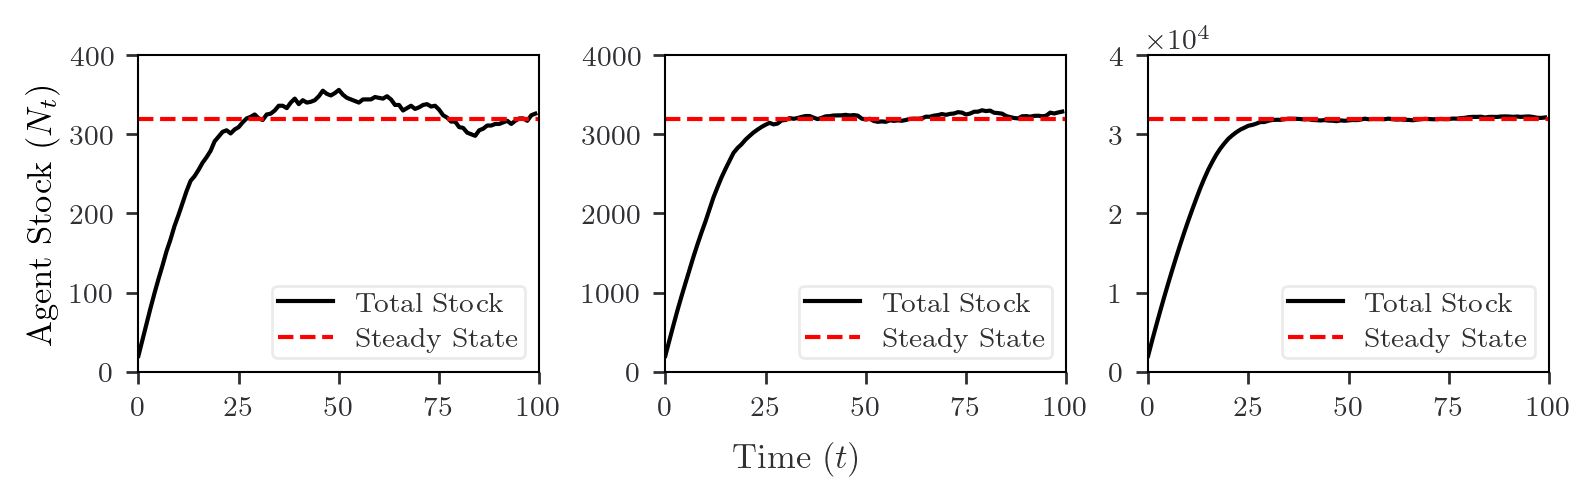
\includegraphics{abm-conv-ssize.png}
    \label{fig:abm-conv-ssize}
\end{figure} 

\subsection{Myopic Best-Response Dynamics}
Finally, I simulate the SBDP market under myopic best-response dynamics \citep{fudenberg1998theory} to explore whether if SSE can be attained using a more robust process of gameplay. 
For this simulation, agents re-compute their optimal policies at the start of every time period given the current market state, unlike in the previous scenario where optimal policies are computed once with respect to the SSE for some given exogenous settings. 
This process is \textit{myopic} in the sense that agent policies account only for the current platform state but not for its dynamic evolution; yet it is still more robust than the previous experiment as echoing feedback between policy and state updates could create outward-spiralling dynamics that prevent convergence onto SSE. 
The results of these simulations over 120 time periods are presented in \autoref{fig:abm-br}, showing that, both in the case of balanced and unbalanced markets, the SSE can be attained using myopic best response dynamics.

\begin{figure}[ht] 
    \centering
    \caption{Agent-Based Simulation Under Myopic Best Response Dynamics}
    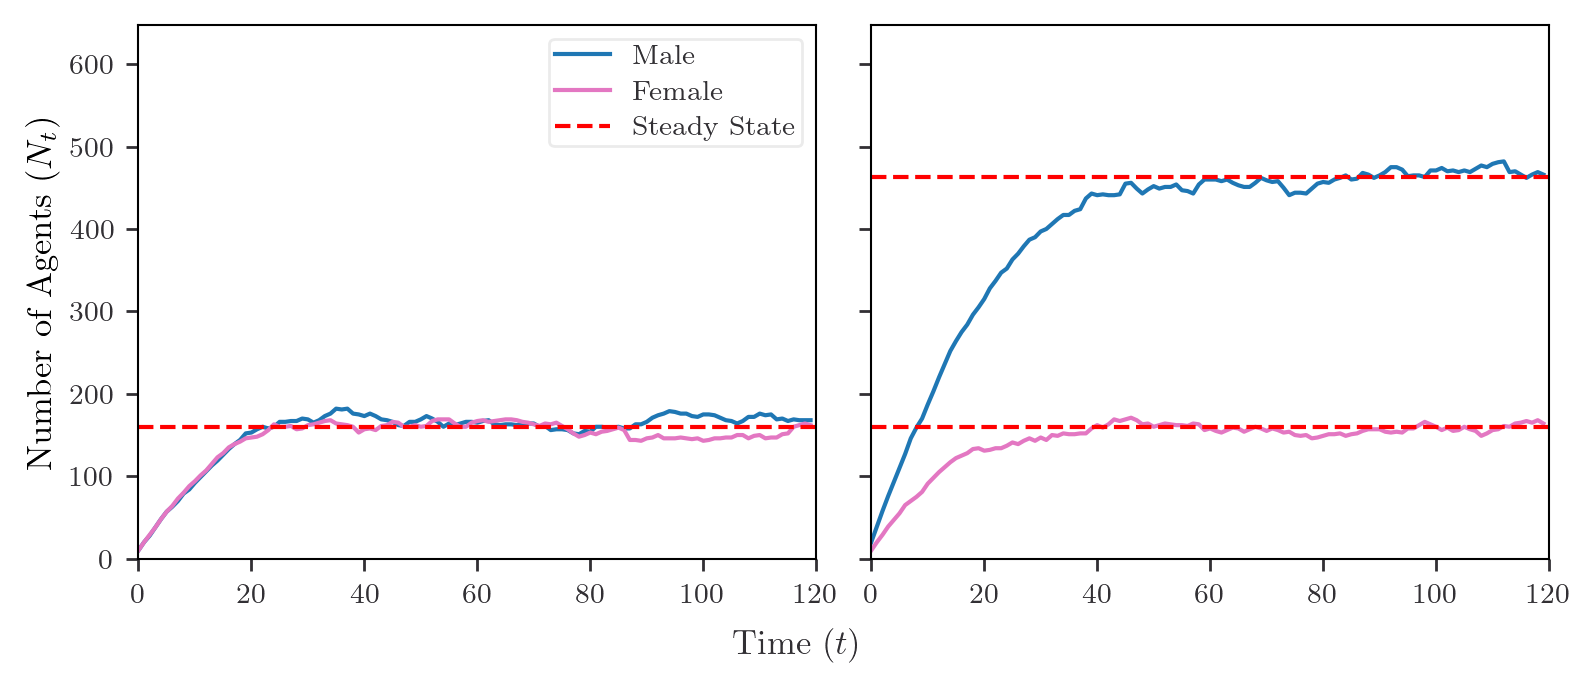
\includegraphics{abm-br.png}
    \label{fig:abm-br}
\end{figure}  


 
\section{Conclusion}
\label{sec:section5}
This paper studied the strategic behaviour of users in SBDP markets by formulating a model of two-sided search for agents with heterogeneous preferences and intertemporal action constraints. 
Using mean-field assumptions that hold for large markets, I provided an explicit characterisation of agent best-responses and used computational procedures to approximate SSE, exploring the effects of different exogenous parameters on both individual behaviour and the aggregate SBDP market.
Finally, I used ABM techniques to asses the convergence properties of my model, as well as its robustness under myopic best-response dynamics, to determine if equilibria can be attained under relaxed gameplay conditions.
I placed particular focus on explaining how the `Fast-Swiping Men' phenomenon can arise in unbalanced markets due to the endogenous relation between an agent's patience, their swiping behaviour, and the market steady state. 
Crucially, I identified that this puzzle is most likely the result of exogenous differences in sex-specific arrival flows, which can be counterbalanced with opposite differences in their respective swiping caps. 
Nevertheless, an interesting direction for future research could involve studying why these inflow differences occur in the first place, perhaps by considering an endogenous relation with competing SBDPs and alternative romantic search markets. 

Overall, this work uncovers a number of actionable insights that could allow SBDPs to enhance both their user experience and their profitability.
The most direct application of these probably involves subscription pricing, since the main benefits that Tinder provides for its paid subscribers include: unlimited swipes, increased visibility, and the ability for an agent to observe profiles that have already liked them \citep{web:tinder_subscription}.
These benefits essentially equate to removing the three sources of search frictions explored by this paper: swiping constraints, market tightness, and strategic considerations, respectively.
As such, the conclusions outlined above could provide guidance to future research, for example, by motivating subscription pricing models that discriminate based on market tightness.
On a final note, one of the main benefits of the model presented in this paper is perhaps its flexibility, admitting to a number of potential extensions that could be used to study more focused aspects of SBDPs. 
One modification of particular interest would involve a richer action set that allows for both multiple casual matches and a single long-term match (after which agents leave the market permanently), which might uncover interesting insights on romantic incompatibility and associated search frictions in SBDPs.

\pagebreak

\addcontentsline{toc}{section}{References}
\bibliographystyle{apalike}
\bibliography{references}

\begin{appendices}
\addcontentsline{toc}{section}{Appendix}
\section{Solving For The Market Steady State}

\label{appx: Flux Sketch} 
\section{Proof for Proposition 1}
\label{appx: b} 
To prove Proposition 1, we rely the following two equations; the first of which expresses the agent's value function in piecewise form, and the second of which describes the necessary condition for all reservation attractiveness values:

\begin{equation}\label{eq:A.1}
    V(\theta, b)=\begin{cases} 
        \overline\mu u(\theta) +\alpha \,\mathbb{E}_{\theta}\Big[V(\theta', b-1)\Big],& \theta> \widetilde \mu_b \\[10pt]
        \alpha \,\mathbb{E}_{\theta}\Big[V(\theta', b)\Big],& \theta\leq\widetilde \mu_b
    \end{cases}  
\end{equation}\\


\begin{equation}\label{eq:A.2}
    \overline\mu u(\widetilde\omega_b) = \alpha \, \mathbb{E}_\theta\Big[\,V(\theta',b)-V(\theta',b-1)\,\Big]  
\end{equation}
 
To simplify notation, denote the continuation value at budget $b$ by:

\begin{equation*}
    \begin{aligned}
        &K_{b}:=\alpha \,\mathbb{E}_{\theta}\left[V(\theta', b)\right] 
    \end{aligned} 
\end{equation*}

Starting out with \autoref{eq:A.2} and expanding out the expectation operator, we can use \ref{eq:A.1} to substitute in the piecewise definitions of $V(\theta,b)$ over the appropriate intervals:

\begin{equation}\label{eq:A.3}
    \begin{split}
        \overline\mu u(\widetilde\omega_b) &= \alpha \,\int^1_0\,V(\theta',b)-V(\theta',b-1)\,dF_m(\theta')\\
                                           &=\alpha \int^{\widetilde\omega_b}_0\,K_b\,dF_m(\theta') \,+\, \alpha \int^1_{\widetilde\omega_b}\,\overline\mu u(\theta') + K_{b-1}\,dF_m(\theta')\\ 
                                           & \quad -\,\alpha \int^{\widetilde\omega_{b-1}}_0 K_{b-1}\,dF_m(\theta') \,-\, \alpha \int^1_{\widetilde\omega_{b-1}} \overline\mu u(\theta') + K_{b-2}\,dF_m(\theta')
    \end{split}
\end{equation}

Furthermore, Equation \ref{eq:A.2} implies that:

$$
\overline\mu u(\widetilde\omega_b) +K_{b-1}= K_b
$$

$$
\overline\mu u(\widetilde\omega_{b-1}) +K_{b-2}=K_{b-1}
$$

Then, by substituting these expressions into \ref{eq:A.3}, we arrive at \ref{eq:A.4}:

\begin{equation}\label{eq:A.4}
    \begin{split}
        \overline\mu u(\widetilde\omega_b) &=\alpha \int^{\widetilde\omega_b}_0\,\overline\mu u(\widetilde\omega_b) +K_{b-1}\,dF_m(\theta') \,+\, \alpha \int^1_{\widetilde\omega_b} \,\overline\mu u(\theta') + K_{b-1}\,dF_m(\theta')\\ 
                                           & \quad -\,\alpha \int^{\widetilde\omega_{b-1}}_0 K_{b-1}\,dF_m(\theta') \,-\, \alpha \int^1_{\widetilde\omega_{b-1}} \overline\mu u(\theta') + K_{b-1}-\overline\mu u(\widetilde\omega_{b-1})\,dF_m(\theta')
    \end{split}
\end{equation}

With some algebra, this simplifies down to the recurrence relation in \autoref{eq:recurrence relation}: 

\begin{equation}
    u(\widetilde\omega_b)=\alpha   u(\widetilde\omega_b)F_m(\widetilde\omega_b) \,  \,+\,\alpha  u(\widetilde\omega_{b-1})\Big(1  - F_m(\widetilde\omega_{b-1})\Big) \,+\, \alpha\int^{\widetilde\omega_{b-1}}_{\widetilde\omega_b} u(\theta') \,dF_m(\theta') 
\end{equation}

Furthermore, to obtain the initial condition for the above, we impose the right-swiping budget constraint where $V(\theta,0)=0, \forall b\in \mathcal{B}_w$. Then, \ref{eq:A.1} and \ref{eq:A.2} simplify to:

\begin{equation}\label{eq:A.5}
    V(\theta, 1)=\begin{cases} 
        \overline\mu u(\theta),& \theta> \widetilde \omega_1 \\ 
        \alpha \,\mathbb{E}_{\theta}\Big[V(\theta', 1)\Big],& \theta\leq\widetilde \omega_1
    \end{cases}  
\end{equation}\\ 

\begin{equation}\label{eq:A.6}
    \overline\mu u(\widetilde\omega_1) = \alpha \, \mathbb{E}_\theta\Big[\,V(\theta',1)\,\Big]  
\end{equation}

Beginning with \ref{eq:A.6}, we simplify until arriving at \autoref{eq:initial condition}:

\begin{equation*} 
    \begin{split}
        \overline\mu u(\widetilde\omega_1) &= \alpha \, \mathbb{E}_\theta\Big[\,V(\theta',1)\,\Big]\\
        &= \alpha \,\int^{\widetilde\omega_1}_0\,K_1\,dF_m(\theta') + \alpha \,\int_{\widetilde\omega_1}^1 \overline\mu u(\theta')\,dF_m(\theta')\\
        &= \alpha \,\int^{\widetilde\omega_1}_0\,\overline\mu u(\widetilde\omega_1)\,dF_m(\theta') + \alpha \,\int_{\widetilde\omega_1}^1 \overline\mu u(\theta')\,dF_m(\theta')\\
        &= \alpha \overline\mu u(\widetilde\omega_1)F_m(\widetilde\omega_1) + \alpha \,\int_{\widetilde\omega_1}^1 \overline\mu u(\theta')\,dF_m(\theta')\\
        \implies u(\widetilde\omega_1) &= \alpha u(\widetilde\omega_1)F_m(\widetilde\omega_1) + \alpha \,\int_{\widetilde\omega_1}^1 u(\theta')\,dF_m(\theta') 
    \end{split}
\end{equation*}  

To conclude the proof, note that existence and uniqueness of $\widetilde\omega_b$ satisfying \ref{eq:A.2} are guaranteed given the assumptions on $u(\theta)$ being continuous and strictly increasing. Since continuation values must be strictly bounded between 0 and $u(1)$, then, by the Intermediate Value Theorem, there is only one root $\widetilde\omega_b$ satisfying \ref{eq:A.2}.

\section{Notation}
\label{appx: c notation} 
\begin{itemize}
    \item Male types $\mu$
    \item Female types $\omega$
    \item Strategies $s=(s_m,s_w)$
    \item CDF's $M(\mu, b)$, $W(\omega,b)$
    \item Densities $m(\mu, b)$, $w(\omega,b)$
    \item Discount $\delta$ 
    \item Population CDF's $F_m, F_w$
    \item Masses $N_m, N_w$
    \item Entry Flows $\lambda_m, \lambda_w$
    \item Tightness $\tau = \min\{\frac{N_w}{N_m}, 1\}$
    \item Effective discount $\alpha$ 
\end{itemize}

\end{appendices}
 
\end{document}
